\documentclass[11pt]{article}
\usepackage{geometry}                
\geometry{letterpaper}   
\usepackage[framed, numbered, autolinebreaks]{mcode}                
\usepackage{float}
\usepackage{graphicx}
\usepackage{amssymb}
\usepackage{epstopdf}
%\usepackage{natbib}
\usepackage{amssymb, amsmath}
\DeclareGraphicsRule{.tif}{png}{.png}{`convert #1 `dirname #1`/`basename #1 .tif`.png}

\graphicspath{ {images/} }

%\title{Trail Formation}
%\author{Name 1, Name 2}
%\date{date} 

\begin{document}



\thispagestyle{empty}

\begin{center}
\includegraphics[width=5cm]{ETHlogo.eps}

\bigskip


\bigskip


\bigskip


\LARGE{ 	Lecture with Computer Exercises:\\ }
\LARGE{ Modelling and Simulating Social Systems with MATLAB\\}

\bigskip

\bigskip

\small{Project Report}\\

\bigskip

\bigskip

\bigskip

\bigskip


\begin{tabular}{|c|}
\hline
\\
\textbf{\LARGE{Trail Formation}}\\
%\textbf{\LARGE{...}}\\
\\
\hline
\end{tabular}
\bigskip

\bigskip

\bigskip

\LARGE{Michael Mattmann \& Riccardo Schira}



\bigskip

\bigskip

\bigskip

\bigskip

\bigskip

\bigskip

\bigskip

\bigskip

Zurich\\
December 2014\\

\end{center}



\newpage

%%%%%%%%%%%%%%%%%%%%%%%%%%%%%%%%%%%%%%%%%%%%%%%%%

\newpage
\section*{Agreement for free-download}
\bigskip


\bigskip


\large We hereby agree to make our source code for this project freely available for download from the web pages of the SOMS chair. Furthermore, we assure that all source code is written by ourselves and is not violating any copyright restrictions.

\begin{center}

\bigskip


\bigskip


\begin{tabular}{@{}p{3.3cm}@{}p{6cm}@{}@{}p{6cm}@{}}
\begin{minipage}{3cm}

\end{minipage}
&
\begin{minipage}{6cm}
\vspace{2mm} 

\large Michael Mattmann

 \vspace{\baselineskip}

\end{minipage}
&
\begin{minipage}{6cm}

\large Riccardo Schira

\end{minipage}
\end{tabular}


\end{center}
\newpage

%%%%%%%%%%%%%%%%%%%%%%%%%%%%%%%%%%%%%%%



% IMPORTANT
% you MUST include the ETH declaration of originality here; it is available for download on the course website or at http://www.ethz.ch/faculty/exams/plagiarism/index_EN; it can be printed as pdf and should be filled out in handwriting

\includegraphics[width=\columnwidth]{declaration-originality.png}


%%%%%%%%%% Table of content %%%%%%%%%%%%%%%%%

\tableofcontents

\newpage

%%%%%%%%%%%%%%%%%%%%%%%%%%%%%%%%%%%%%%%



\section{Abstract}

Agent-based models can provide an easily implementable way to study complex systems. As Helbing et al. (1997) have shown, many aspects of pedestrian motion, such as the formation of trail systems in green areas, can be reproduced using a relatively simple “active walker” model that takes into account the attractiveness of terrain and feedback on the terrain as it is walked upon. In the current project, we plan to apply this model, and implement the topology of the ground, so that the decisions of peoples can be simulated more accurately. We plan to simulate some simple and idealized situation, to confirm our model and in the end apply it to a real park without trails (like university campus) and see if the result will be the same as in reality. We plan also to apply our model to a bigger park (e.g. Central Park) with all the existing trails/streets and see what would change if peoples can choose in which direction the want to go, without being obligated by tarred streets. 

In a first step we are going to implement the model like described in the literature and implement our additions, we will than determine if this model is suitable also to not flat grounds by testing it on some scenarios. 
In a second step, we will determine the efficiency of already existing trail networks, and see how they would change in time, if they are free to. 

We expect to find that in small university campus, natural crated trails will correspond quite well with our model, while parks in cities, with tarred streets will differ in some manner from our results. We suggest that this is caused by the fact that park are not only use to go from a place to an other but also to simply take a walk and therefore not the most direct way is chosen by pedestrian.

\section{Individual contributions}

The whole project was completed as a team. Since we decided to do this work only in two, both contributed to the implementation of the model in Matlab, the analysis of the achieved results and in writing the final report.

\newpage 
 
\section{Introduction and Motivations}

\subsection{Introduction}

We want to implement a model that can simulate the behaviour of peoples while walking on an open space. We are going to use the already existing model created from Helbing and add the topology of the ground. We have decided to do so because we think it's an important factor involved in the decision of the direction in which to walk and as it, it should be taken into account while simulating the decision of peoples.  

First we will simulate some simple situation and try to explain the results of them. In the second part we will instead take some real examples and look how people would walked in a park if they decide to use it only as a passage and therefore not to walk any more on the tarred ways.

\subsection{Motivations} 

We wanted to deal with this subject because it can be found in all day life since it influences the look of every park that can be found in a city. 

We decided so also because it seemed to be really interesting as it involves many factors, which can vary from person to person, and therefore the individual trajectory can't be predicted precisely, but the whole set of trails can be predicted well.

\subsection{Fundamental Questions}

After the implementation of our model we are interested in answering the following questions: 

\begin{itemize}
\item How do trajectories form?
\item What is the final network of the most common sets of entrance / exits?
\item How does topology influence the final network?
\item How would the system of trails of a real park change over time if the existing "trails" will be no longer asphalted?
\end{itemize}

In addition we are keen to know if our model is a good abstraction of the reality.

\newpage
\subsection {Expected Results}

Before making computer simulations we discussed, what we expect as results out of the simulation:

\begin{itemize}
\item The planning of real parks will always be influenced from many parameters, like design, financing mechanism, personal interests, etc. Because of this reasons we expect to find some differences between our model and what we can find in cities. 
\item In smaller green spaces, like in some university campus, we expect to find great similarities with what predicted from our model. That because there are no existing tarred streets, and pedestrians are therefore free to chose in which direction they want to walk. 
However in this case we'll find problems in finding information about what are the entrances, exits and haw many peoples are going to pass trough. And because of this also on that case there will be some differences. 
\item There are many parameters we do not model in our simulation. For example the interaction between pedestrians ("social force"), distractions while walking, etc. By leaving out this details we get a very simplified model. However, we think that these parameters will only minimally affect the motion of pedestrians. We hope therefore to get the same a realistic model capable to predict in accurate way the formation of trail systems. 
\end{itemize}

\newpage

\section{Description of the Model}

The ground idea of the model is not complicated and it includes only a few parameter, but its implementation is more complex, because there are many things that must be considered (boundary condition, ...) and it must be made not in a continuous manner, but discrete. In this section only how the model is and not how it is implemented is going to be explained.

The position of a general point on the floor is indicated by the vector $\vec{r}$. The ground structure  $G(\vec{r},t)$ with  \[\vec{r} =  \left( \begin{array}{ccc}
x\\
y\\    \end{array} \right)\]
is a function which has to contain the information about the presence of trails and its intensity depending on position $r$ and time $t$. We have decided that the intensity of a trail is in the interval $\lbrack 0, 1 \rbrack$: $0$ indicate that there is no trail (natural condition) and $1$ that the ground has reached the maximum possible intensity of trail. 
The trail (it's intensity) on a particular place is the result of the sum of the contributions of all pedestrian that have walked on this place and the regeneration of the ground itself. 
Each pedestrian leave a footprint whit the intensity 
\[I\cdot(1-G(\vec{r},t))\]
with I a parameter which indicates the intensity of the footprint. 
So we can say that the equation which describe the evolution of the ground structure is:
\[\frac{dG(\vec{r},t)}{dt}=-R \cdot G(\vec{r},t)+I\cdot(1-G(\vec{r},t))\sum_p \delta(\vec{r} - \vec{r_p}(t)) \]
with $R$ the parameter for the regeneration ratio,  $\delta()$ the Dirac’s delta function and $\vec{r_p}(t)$ the position of a pedestrian $P$.

\medskip

Another function $T(\vec{r})$ defined by the user has to describe the topology of the ground, i.e., for each point $\vec{r}$ the function associates an altitude. Now that we know the topology for each position we have to explain how the pedestrian choose their trajectories. To do this we have to introduce another function $V_{p}(\vec{r_p},\vec{r},t)$, called the ground potential with respect to the person $P$, which describes the attractiveness of a certain place $\vec{r}$ with respect to the position $\vec{r_p}$ of the person depending on time. The attractiveness of a place depends on two factor: 
\begin{itemize}
\item The presence of tracks in the neighbourhood
\item The slope of the ground between $\vec{r_p}$ and $\vec{r}$
\end{itemize} 
We can say that $V_{p}(\vec{r_p},\vec{r},t)=Z+U_p$, where Z is the part of the potential about the presence of tracks in the neighbourhood of a general place $\vec{r}$ (this part doesn't depend on the position of the person) and $U_p$ is the part of the slope (this instead depends on $\vec{r_p}$).
We consider the presence of trails with the factor
\[G(\vec{r^\prime},t) \cdot \mathrm{e}^{\frac{-\|\vec{r} -\vec{r^\prime}\|}{\sigma}}\]   
(where $\sigma$ is a parameter for the visibility), so that the further a general point $\vec{r^`}$ with tracks $G(\vec{r^`},t)$ is, the less it count.
So we can write 
\[Z(\vec{r},t)=
    \int \!\!\! \int_{Ground} G(\vec{r^\prime},t) \cdot \mathrm{e}^{\frac{-\|\vec{r} -\vec{r^\prime}\|}{\sigma}}\,d\vec{r^\prime} .\]
  The slope of the ground is considered with  \[U_p(\vec{r_p},\vec{r},t)=-\mathrm{e}^{\frac{-\alpha\cdot\|\vec{r}-\vec{r_p}\|}{|T(\vec{r})-T(\vec{r_p})|}},\]
with $\alpha>0$ the parameter for slope.

The direction $\vec{d_p}(t)$ of a pedestrian is also given by the weighted (with a scalar parameter $l$) average of the normalized direction, which indicates the place where the pedestrian want to arrive, and the normalized gradient of the ground potential. In that way if we put the position of the arrival of the pedestrian as $\vec{u_p}$  the direction is 

\[\vec{d_p}(\vec{r_p},t)=\frac{\vec{u_p} -\vec{r_p}(t)}{\| \vec{u_p} -
    \vec{r_p}(t)\|} +l\cdot \frac{\nabla V(\vec{r_p}(t),t)}{\|\nabla 
    V(\vec{r_p}(t),t)\|} \]
Finally we normalize this direction obtaining
\[\vec{e_p}(\vec{r_p},t)=\frac{\vec{d_p}(t)}{\|\vec{d_p}(t)\|} \]
in this way we can write the equation of motion of a pedestrian as 
\[\frac{d\vec{r_p}(t)}{dt}=v_p\cdot \vec{e_p}(\vec{r_p},t) \]
with $v_p$ the speed with which the pedestrian is walking. 
\newpage


\section{Implementation}

\subsection{General}

As I already said although the model is continuous its implementation on Matlab is done in a discrete manner, so all the function depending on the position are in the code matrix with the dimension dm$\times$ dn. We decided that a cell of the matrix represent 1 m$^{2}$ of the ground, so dm and dn are lenght and the large in m of the rectangular field that is considered. Initially we decided that a cell of the matrix was 50cm$\times$50cm to have a high resolution, but the simulations took very long time to be computed, therefore we had to take a compromise. The most important matrix in the code are:
\begin{itemize}
\item G2: The ground structure (G in the description of the model). Each cell has the value of the intensity of its own track.
\item G4: the potential of the ground depending only on the presence of tracks in the neighbourhood (Z in the description). Each cell has the value of its own potential.
\item pot$\_$per: the total potential ($V_{p}$ in the description)
\item G1: the topology (T in the description). Each cell has the value of its own altitude.
\end{itemize} 
\subsection{Scripts}
The model is composed essentially by 6 scripts:
\begin{itemize}
\item 'start.m' in which we can set the parameters and the number of entrances/exits and their position for various simulations. This is also the script that has to been executed in order to make a simulation, because it recall the main script. 
\item 'main.m' in which the actual simulation take place. Here the variables that were not already been initialised in 'start.m' are defined and the main loop is implemented. The main loop contain the 4 remains scripts and the code for plotting (and capturing) the matrix G2 in order to take a video of the evolution of the ground structure.
\item 'change\_ground.m' that changes the intensity of the presence of tracks in cells. This is done when a person is on a cell and due to the regeneration ratio of the nature.
\item 'insert\_person\_N\_entrance\_N\_exit.m' that randomly (but with a certain probability) insert a person in one of the N entrances and decide which is his arrival (one of the N exits is chosen).
\item 'direction\_pend.m' that compute which is the best direction for each person. This is the most complex script in the implementation, therefore in the next subsection a more detailed explanation is given.
\item 'move\_person.m' that simply if the pedestrian is not already arrived to his target moves him, else he is deleted.
\end{itemize} 
\subsection{Explanation of 'direction\_pend.m'}
The code in this script is dived in two parts: the first compute $Z$ and the second compute $V_p$ and $\vec{e_p}$. In figure \ref{part1} the code of the first part.
\begin{figure}[h]
\begin{lstlisting}
for aa=1 : dm   % for that goes trough the matrix
    for bb=1:dn
        pottot=0; % Sum of all potentials with respect to point [aa bb]
        for q=1:dm
            for w=1:dn
                if (M(q,w,2)~=0)
                    pot = M(q,w,2)*exp(-((aa-q)^2 + (bb-w)^2)^(1/2)/sigma);% Potential of the ground in [q w] respect to [aa bb]
                    pottot=pottot+ pot; % Sum
                end
            end
        end
        pottot = pottot/(dm*dn); % Avarage
        M(aa,bb,4)=pottot; % Putting the potential in the matrix crated for it  
    end
end
\end{lstlisting}
\caption{First part of code of 'direction\_pend.m'}
\label{part1}
\end{figure}
As i already said the implementation is discrete,therefore the surface integral is here a sum over all the columns and all the  rows: the for at line 5 e 6 go through the matrix, line 6 check if the ground potential at point (q,w) is not 0 (this isn't necessary but it increase the performance, because if it is 0 it's useless to compute line 7), line 7 compute the factor $G(\vec{r^\prime},t) \cdot \mathrm{e}^{\frac{-\|\vec{r} -\vec{r^\prime}\|}{\sigma}}$ and line 8 does the sum. Line 12 divide the sum by the total area of the matrix so that the sum didn't depend on the matrix and line 13 simply put the result in the matrix of the first part of the potential (in the description Z). This must be done for each cell, because the potential is defined overall, so the loops at line 1 and 2 go through the whole matrix. 

The second part of the script is with respect to the position of each person $P$, so the for at line 1 goes through all the people. The code of this part is in figure \ref {part2}.

The code from line 6 to line 18 compute the factor $U_p(\vec{r_p},\vec{r},t)=-\mathrm{e}^{\frac{-\alpha\cdot\|\vec{r}-\vec{r_p}\|}{|T(\vec{r})-T(\vec{r_p})|}}$ and does the sum $V_{p}(\vec{r_p},\vec{r},t)=Z+U_p$ (at line 10 or 12 depending on the sign of the slope). Here $V_p$ is the matrix pot\_per. This must be done for the hole matrix so the two for at line 4 and 5 go through the matrix. After $U_p$ is computed its gradient and norm are calculated (at line 21 and 22). Then  for the people that are not arrived at destination (the distance from destination is calculated at line 23) the normalized vector of the direction is computed in the last part of the code. the code from line 34 to 36 delete the people already arrived at destination.


\begin{figure}[H]
\begin{lstlisting}
for n=1:num_per  % for all peoples
    if (P(n,5)==0)  % peoples that are not "cancelled"
        pot_per = M(:,:,4);
        for q=1:dm
            for w=1:dn
                dist = ((P(n,1)-q)^2 + (P(n,2)-w)^2)^(1/2); %distance
                if (dist ~=0)
                    pend = (1000*M(q,w,1) - M(P(n,1),P(n,2),1))/dist; %slope
                    if (pend < 0)
                        pot_per(q,w) = M(q,w,4) - exp(1/pend);
                    elseif (pend > 0)
                        pot_per(q,w) = M(q,w,4) - exp(-1/pend);
                    else
                        pot_per(q,w) = M(q,w,4);
                    end
                else
                    pot_per(q,w) = M(q,w,4);
                end
            end
        end
        [fy,fx]=gradient(pot_per(:,:));  % gradient of the potential matrix
        gradnorm = ((fx(P(n,1),P(n,2)))^2 + (fy(P(n,1),P(n,2)))^2)^(1/2);
        distmeta=((P(n,3) - P(n,1))^2 + (P(n,4) - P(n,2))^2)^(1/2);
        if (distmeta ~= 0)
            if (gradnorm ~= 0)
                ex = (P(n,3) - P(n,1))/distmeta + fx(P(n,1),P(n,2))*l/gradnorm;
                ey = (P(n,4) - P(n,2))/distmeta + fy(P(n,1),P(n,2))*l/gradnorm;
            else
                ex = (P(n,3) - P(n,1))/distmeta;
                ey = (P(n,4) - P(n,2))/distmeta;
            end
            norm = (ex^2 + ey^2)^(1/2);
        else
            M(P(n,1),P(n,2),3) = 0;
            clearvars P(n);
            P(n,5)=1;
        end
        ealfa(n,:) = [ex/norm,ey/norm]; % direction vector
    end
end
\end{lstlisting}
\caption{Second part of code of 'direction\_pend.m'}
\label{part2}
\end{figure}

\section{Simulation Results and Discussion}
\subsection{Idealized cases of trail formation}
\subsubsection{Creation of simple geometries}

The first simulation we decided to make, were these with already existing results, so that we could compare our results whit the "correct" ones. 

We began whit different types of "squares" with four entrances and four exits. We chose the possibility of entering at an entrance to be the same for each of the four, and the same fore the exits.
In that way we covered all possibles ways with the same probability. 

\begin{figure}[H]
        \centering
        \includegraphics[width=10cm]{Quadrati.jpg}
        \caption{Two simulations with the same set of four entrance/exit but one rotated 45 degrees on a 70x70 m field}
\end{figure}

The achieved results (see above) matched whit the expected ones already after only 2000 iteration. 

This trajectory are the result of the compromise of two fact:
\begin{itemize}
\item the lenght of the road traveled from each pedestrian from his entry to the exit has to be minimized,
\item for a pedestrian it's better to walk on an already existing trail.
\end{itemize}

\medskip 

For the second performed simulation we chose a "triangle", three entrances, three exits, and all of them with the same probability. 

\begin{figure}[H]
        \centering
        \includegraphics[width=\columnwidth]{Triangolo.jpg}
        \caption{Simulations whit a triangle}
        \label{tr}
\end{figure}

\begin{figure}[H]
        \centering
        \includegraphics[width=5cm]{Expected_Triangle.png}
        \caption{Expected Result of the simulation of the "triangle"}
        \label{exp_tr}
\end{figure}

The results were quite different from what we expected. After the first simulation we confirmed that the model was implemented in the correct way, so we expected to find a similar result also in this case, where the trails are going to encounter in the center of the matrix (see figure [\ref{exp_tr}]). 

Instead of what we expected, after the first 2000 iterations, we saw the result represented in the middle of figure [\ref{tr}]. The first thought was, there is an error, but all other simulations worked good, so we made another simulation, and after 8000 iterations we became the result shown in last image. In that we can see that the "circle" in the middle is slowly becoming smaller.

 We think that the result has this "strange" form, because our model do not consider the inertia of the pedestrian (i.e. that nobody in a normal walk turns suddenly), therefore when the pedestrian reaches the point when his currently trajectory is no more convenient he simply turns in an other one.

\subsubsection{Trail formation with already existing trails}

One simulation performed with an already existing trail on it is represented in the image below. 
We took a straight trail and putted the exit on another side of the matrix. 

\begin{figure}[H]
        \centering
        \includegraphics[width=\columnwidth]{strada.jpg}
        \caption{Simulations whit existing trail}
\end{figure}

The result is exactly what we expected. At the beginning the people follow the existing trail, because it seems easier, but after some iterations, when on the trail which is not used the regeneration of nature begins to become visible, they chose a more direct way. And so at the and we can find an almost straight trail that link directly the entrance with the exit. 
We suppose that waiting a couple more iterations the trail will become perfectly straight. 

\subsubsection{Trail formation on a not flat ground}

As we see in figure [\ref{Slope}] the model with the implementation of the topology work quite well. In this simulation was set that the pedestrian entered in the right respectively left entrance could only go to the right respectively left exit and the topology is shown in the fourth picture. In the first image we can see the simulation after only a few iteration, note that the pedestrian tend to walk on the level lines. The second image show the result after 2000 iterations: the to ways are more close together due to the fact that they are attracted to each other. In the third image (after 5000 iteration) a compromise between the level lines and the attractiveness is reached and the trails are stable.

\begin{figure}[H]
\includegraphics[width=17cm]{slope.jpg}
\caption{Simulation with topology}
\label{Slope}
\end{figure}

\subsection{Simulations on a real Park}
To answer our last question we simulated the behavior of our model on some real parks. In this part of our work we encountered some problems: after having started the first simulation with a small part of Central Park we saw that our model was too slow for such a big Matrix, it took hardly an hour to make only one iteration. 
The search for a new Park wasn't so easy: all parks found in cities were too big or not appropriate for our purpose (for example there were buildings in the middle or some others obstacle like a river)
\subsubsection{Green Park in London}
After a few days of performance improvement of the implementation of the model the simulation speed had doubled so we decided to take some pieces of Green Park (situated in London). 

Figure [\ref{GreenPark}] illustrates the entire Park with existing Trail-Systems. The red rectangles shows wich pieces of this Park we took for our simulations.  

The obtained results were quite interesting. The first simulation (see figure [\ref{GreenPark1}]) went quite how expected, peoples began to walk along the existing streets, but chose in the end a different trail system wich is definitely shorter than the initial one. 

\begin{figure}[H]
        \centering
        \includegraphics[width=\columnwidth]{GreenPark.png}
        \caption{GreenPark}
        \label{GreenPark}
\end{figure}


\begin{figure}[H]
        \centering
        \includegraphics[width=\columnwidth]{GreenPark1.jpg}
        \caption{Simulation 1}
        \label{GreenPark1}
\end{figure}

The second one (see figure [\ref{GreenPark2}]) was instead quite surprising. Already at the beginning of the simulations peoples wer not following the streets, instead they began to form new trails that were quite different from the initial ones. 

We could explain these results only in two different ways:
\begin{itemize}
\item The part of Park, used in the first simulation, was better planned and therefore also the one chosen from the peoples in our simulation. 
\item We had only luck, because in the end the obtained results are in both cases similar to each other. 
\end{itemize}

\begin{figure}[H]
        \centering
        \includegraphics[width=\columnwidth]{GreenPark2.jpg}
        \caption{Simulation 2}
        \label{GreenPark2}
\end{figure}

\subsubsection{Joyce Kilmer Park in Manhattan}
We found than also some simpler and smaller Parks to use for our simulations. One of these is the Joyce Kilmer Park (see the trail network in fig.[\ref{Joyce_Park}]). 

\begin{figure}[H]
        \centering
        \includegraphics[width=\columnwidth]{Joyce_Park.jpg}
        \caption{Joyce Park}
        \label{Joyce_Park}
\end{figure}

Also for this park we were not able to find datas about the percentage of peoples entering at each entrance, respectively using the different exits. We therefore chose a logical option, on the left part, where there are three entrances/exists in a small area we chose to use a smaller probability to appear or go to. The same for the three entrances on the top of the image (for exact datas see in the .m file). 

\begin{figure}[H]
        \centering
        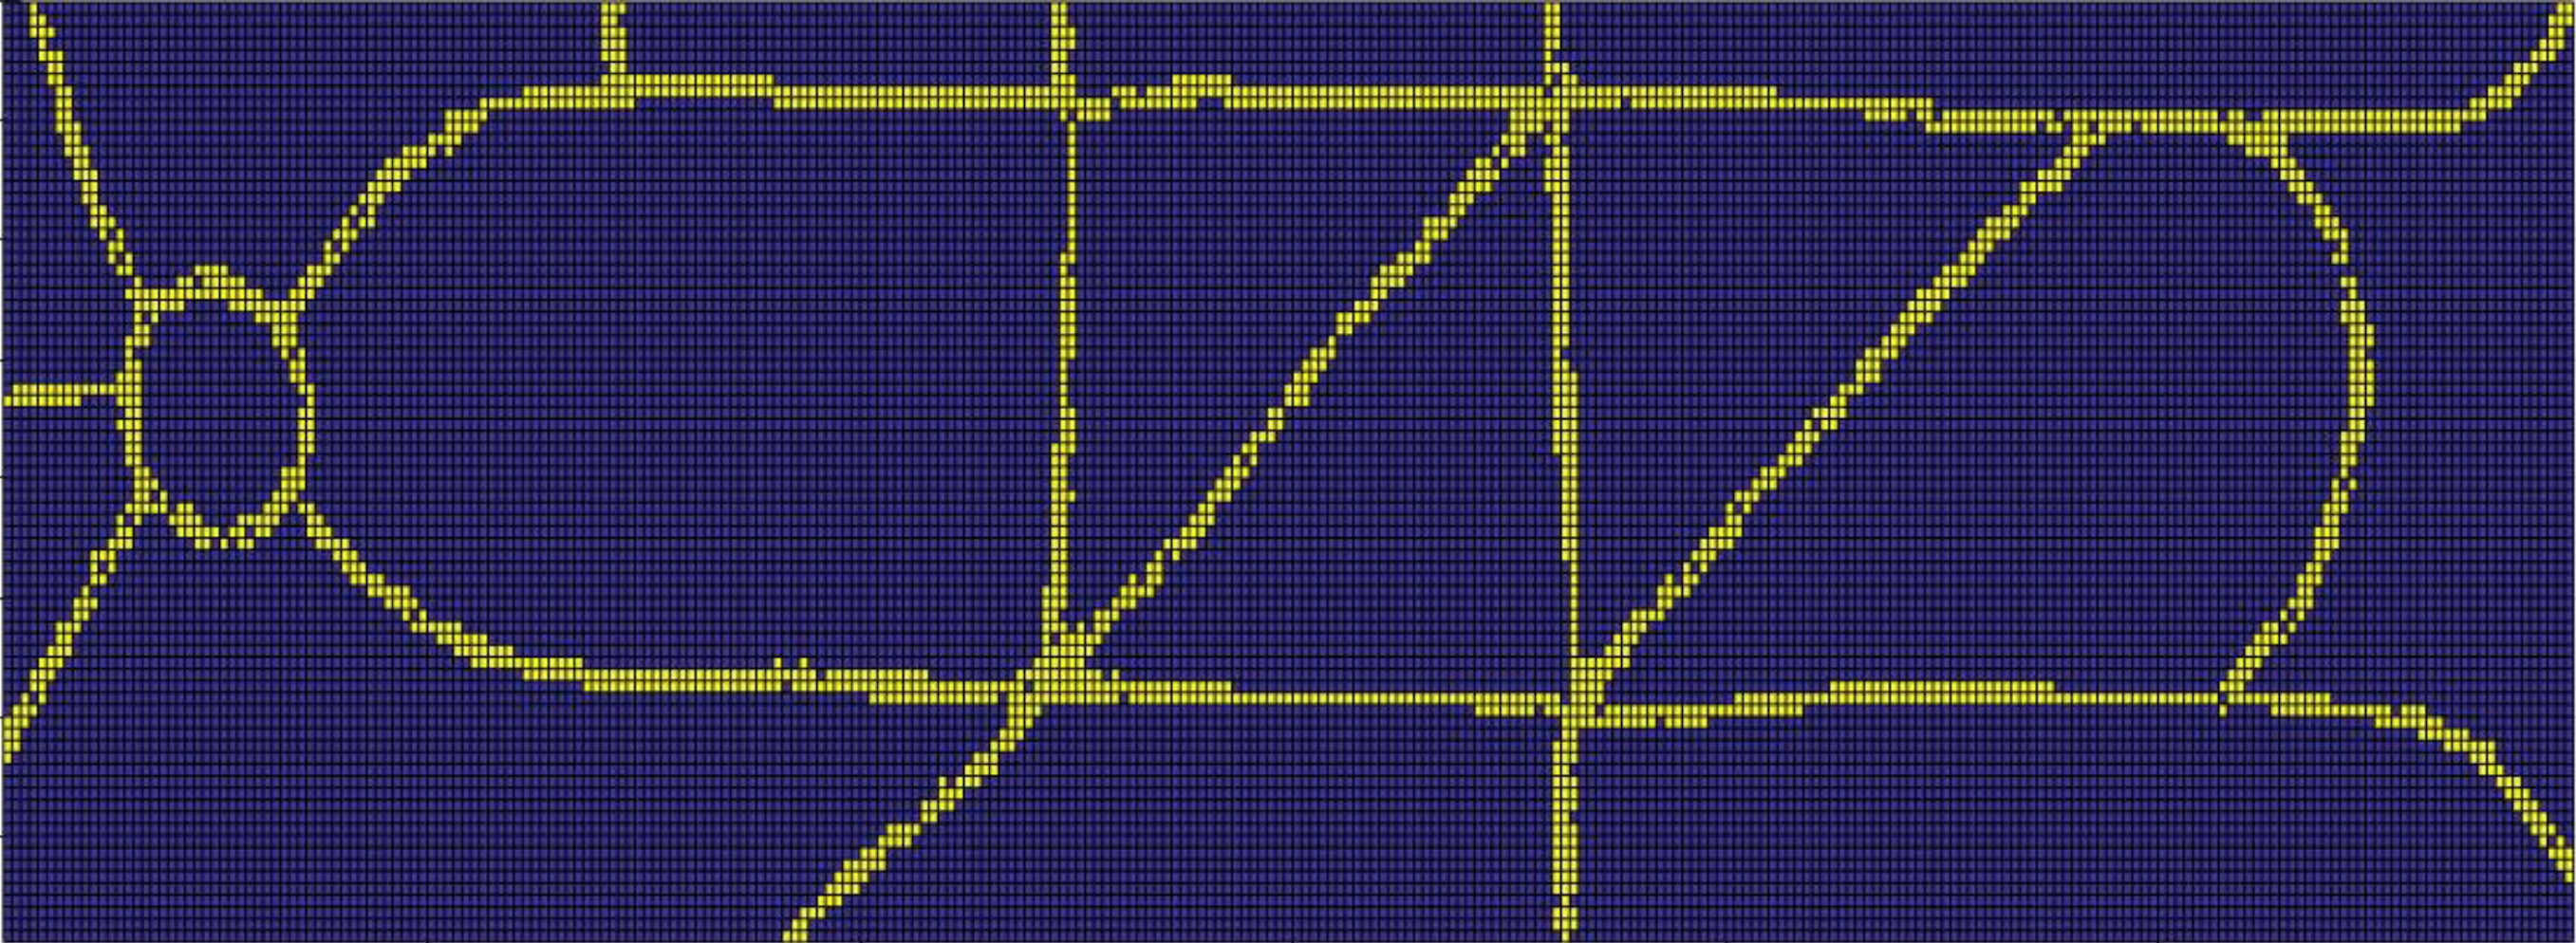
\includegraphics[width=\columnwidth]{jp1.png}
        \caption{Simulation on Joyce Park at the beginning}
        \label{jp1}
\end{figure}

We chose to make a simulation with $10'000$ iterations. 
At the beginning peoples chose to walk along the existing network. This went on up to approximately $1'000$ iterations, after that they begin to chose their own ways across the Park. In fig. [\ref{jp2}] we can see how the first ones began to chose the new ways. 

We notated that the first change appeared in the region of the round on the left side of the Park. This modification seems quite logical, but in reality impossible because of a fountain in the center of that round. Unfortunately we were not able to implement a model that includes the possibility of declaring a "black zone" were peoples should not be able to go. 

\begin{figure}[H]
        \centering
        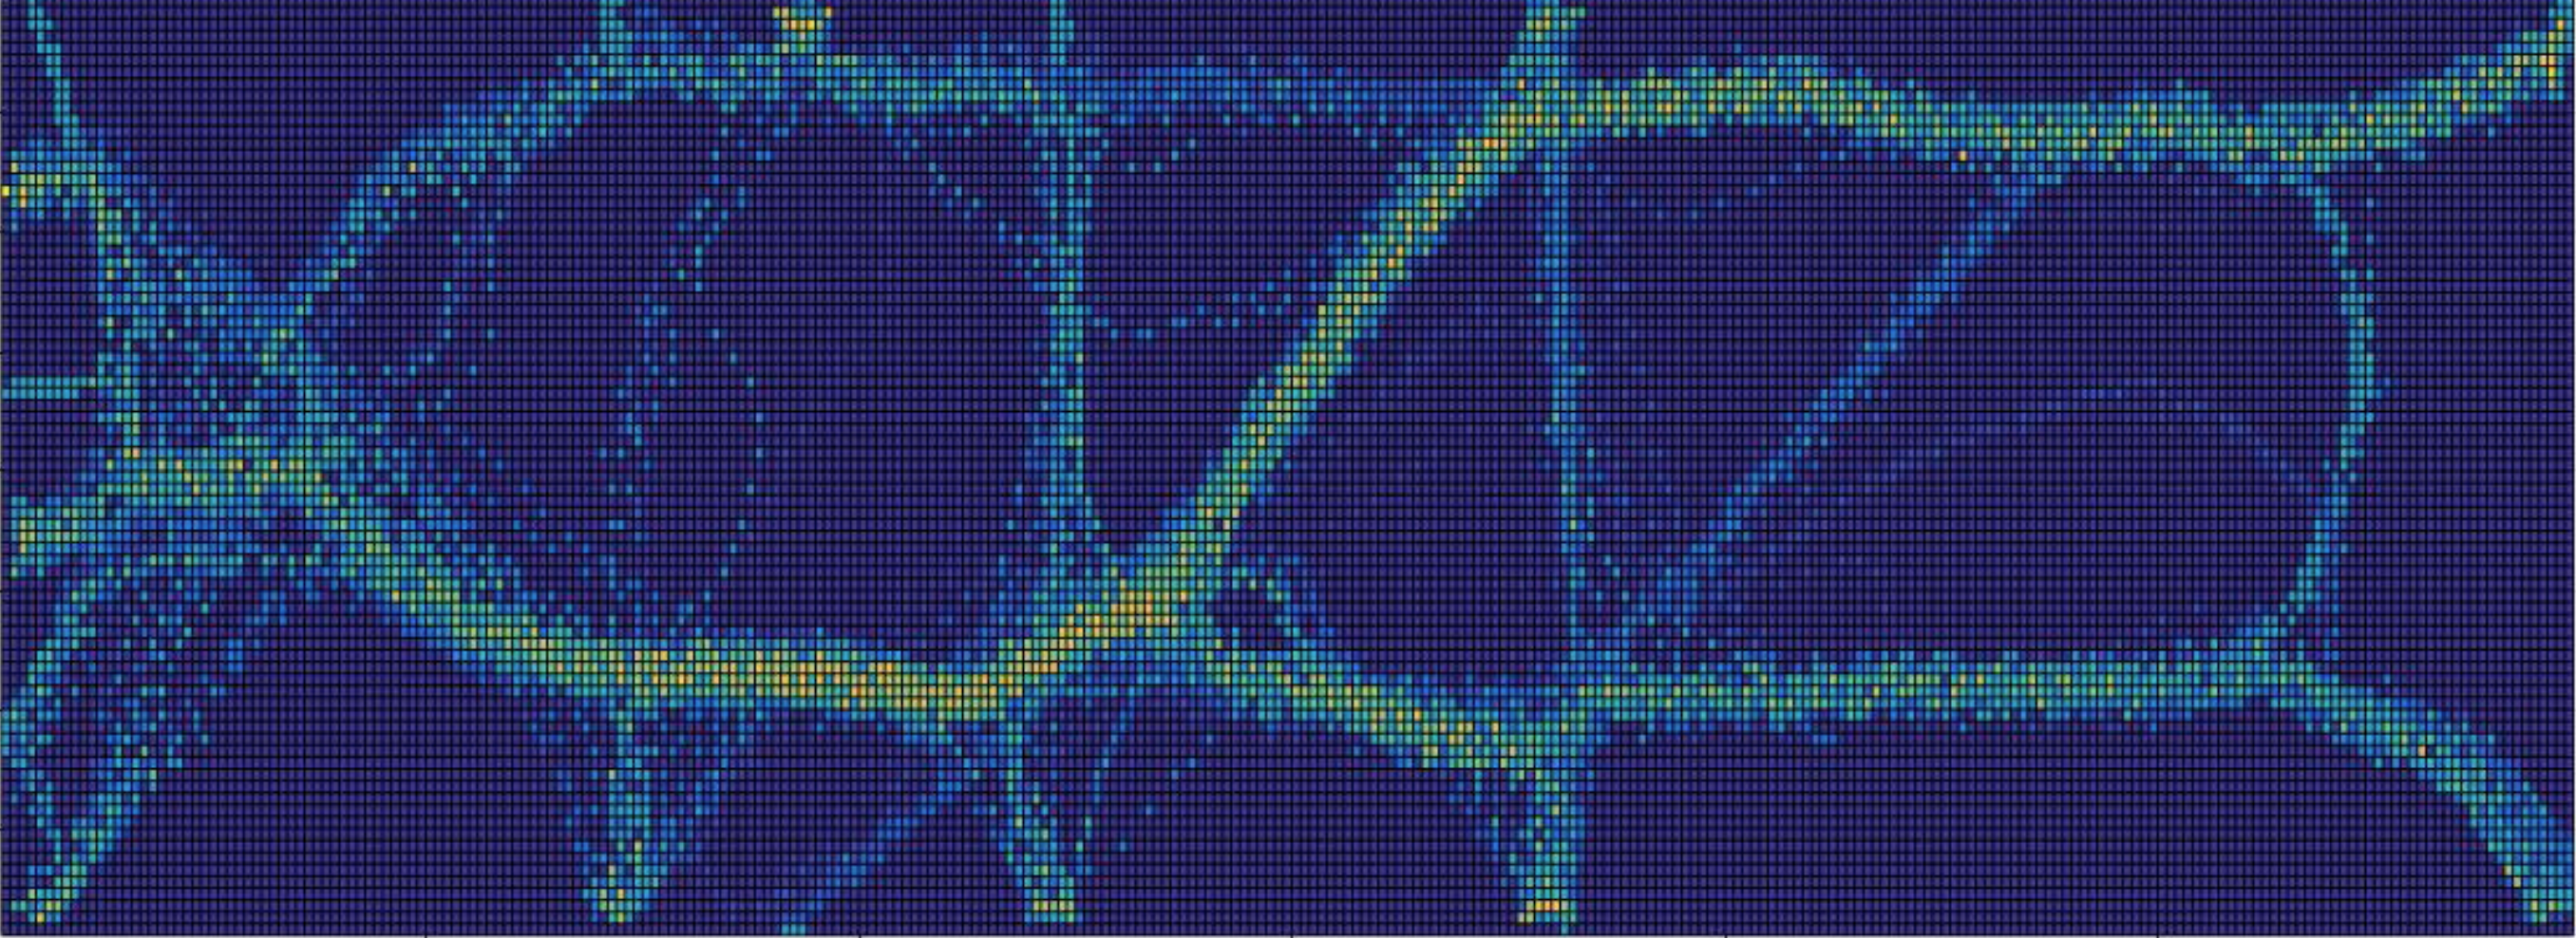
\includegraphics[width=\columnwidth]{jp2.png}
        \caption{Simulation on Joyce Park after 2000 iterations}
        \label{jp2}
\end{figure}

After another $3'000$ iterations on the right part of the Trail network changed only the diagonal street, while on the left already the complete network had changed, the initial "rectangle" already become a single street with some arms connecting the entrances/exits. We suppose that this is due to the faster change at the beginning. 

\begin{figure}[H]
        \centering
        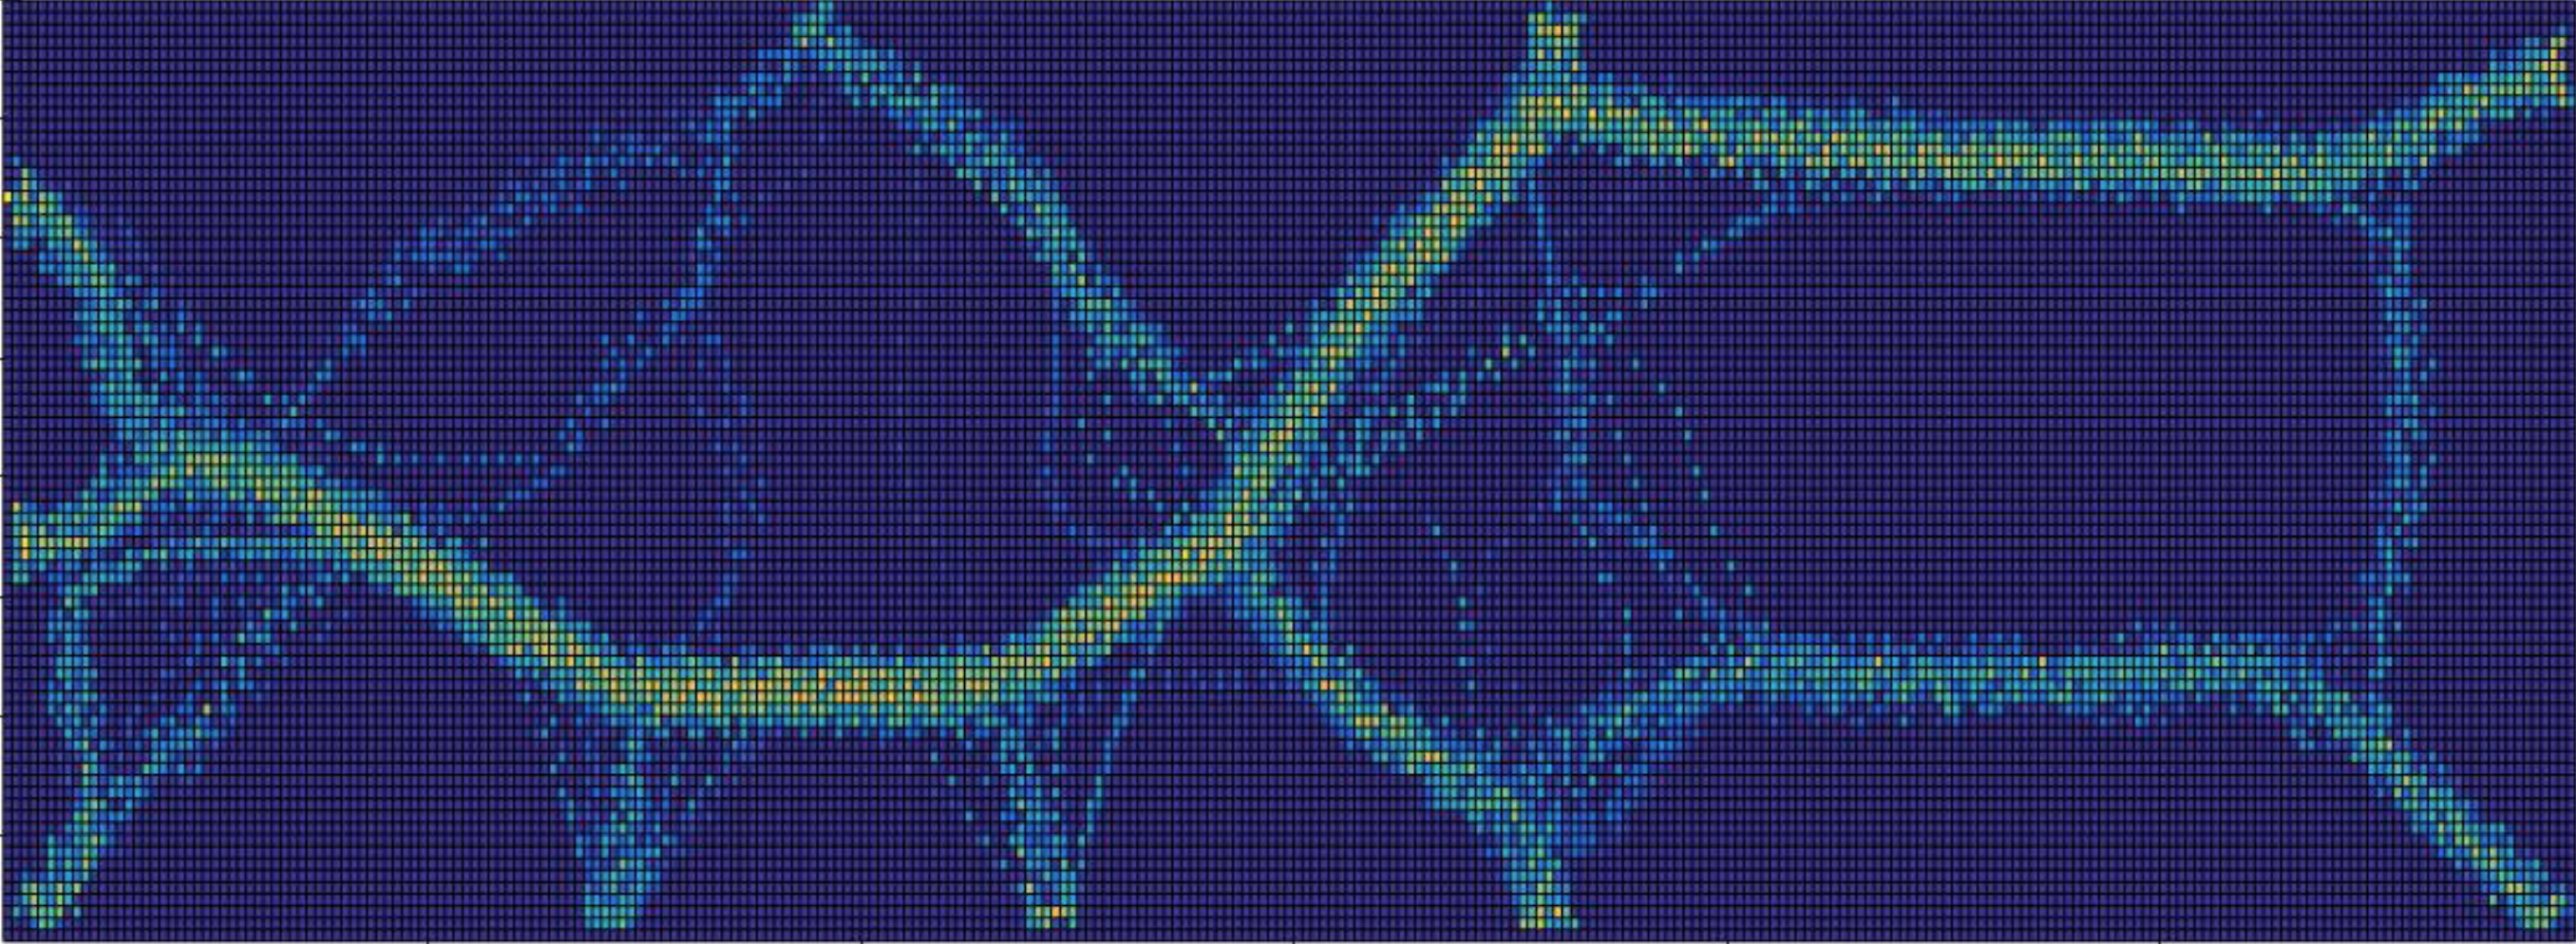
\includegraphics[width=\columnwidth]{jp3.png}
        \caption{Simulation on Joyce Park after 5000 iterations}
        \label{jp3}
\end{figure}

\begin{figure}[H]
        \centering
        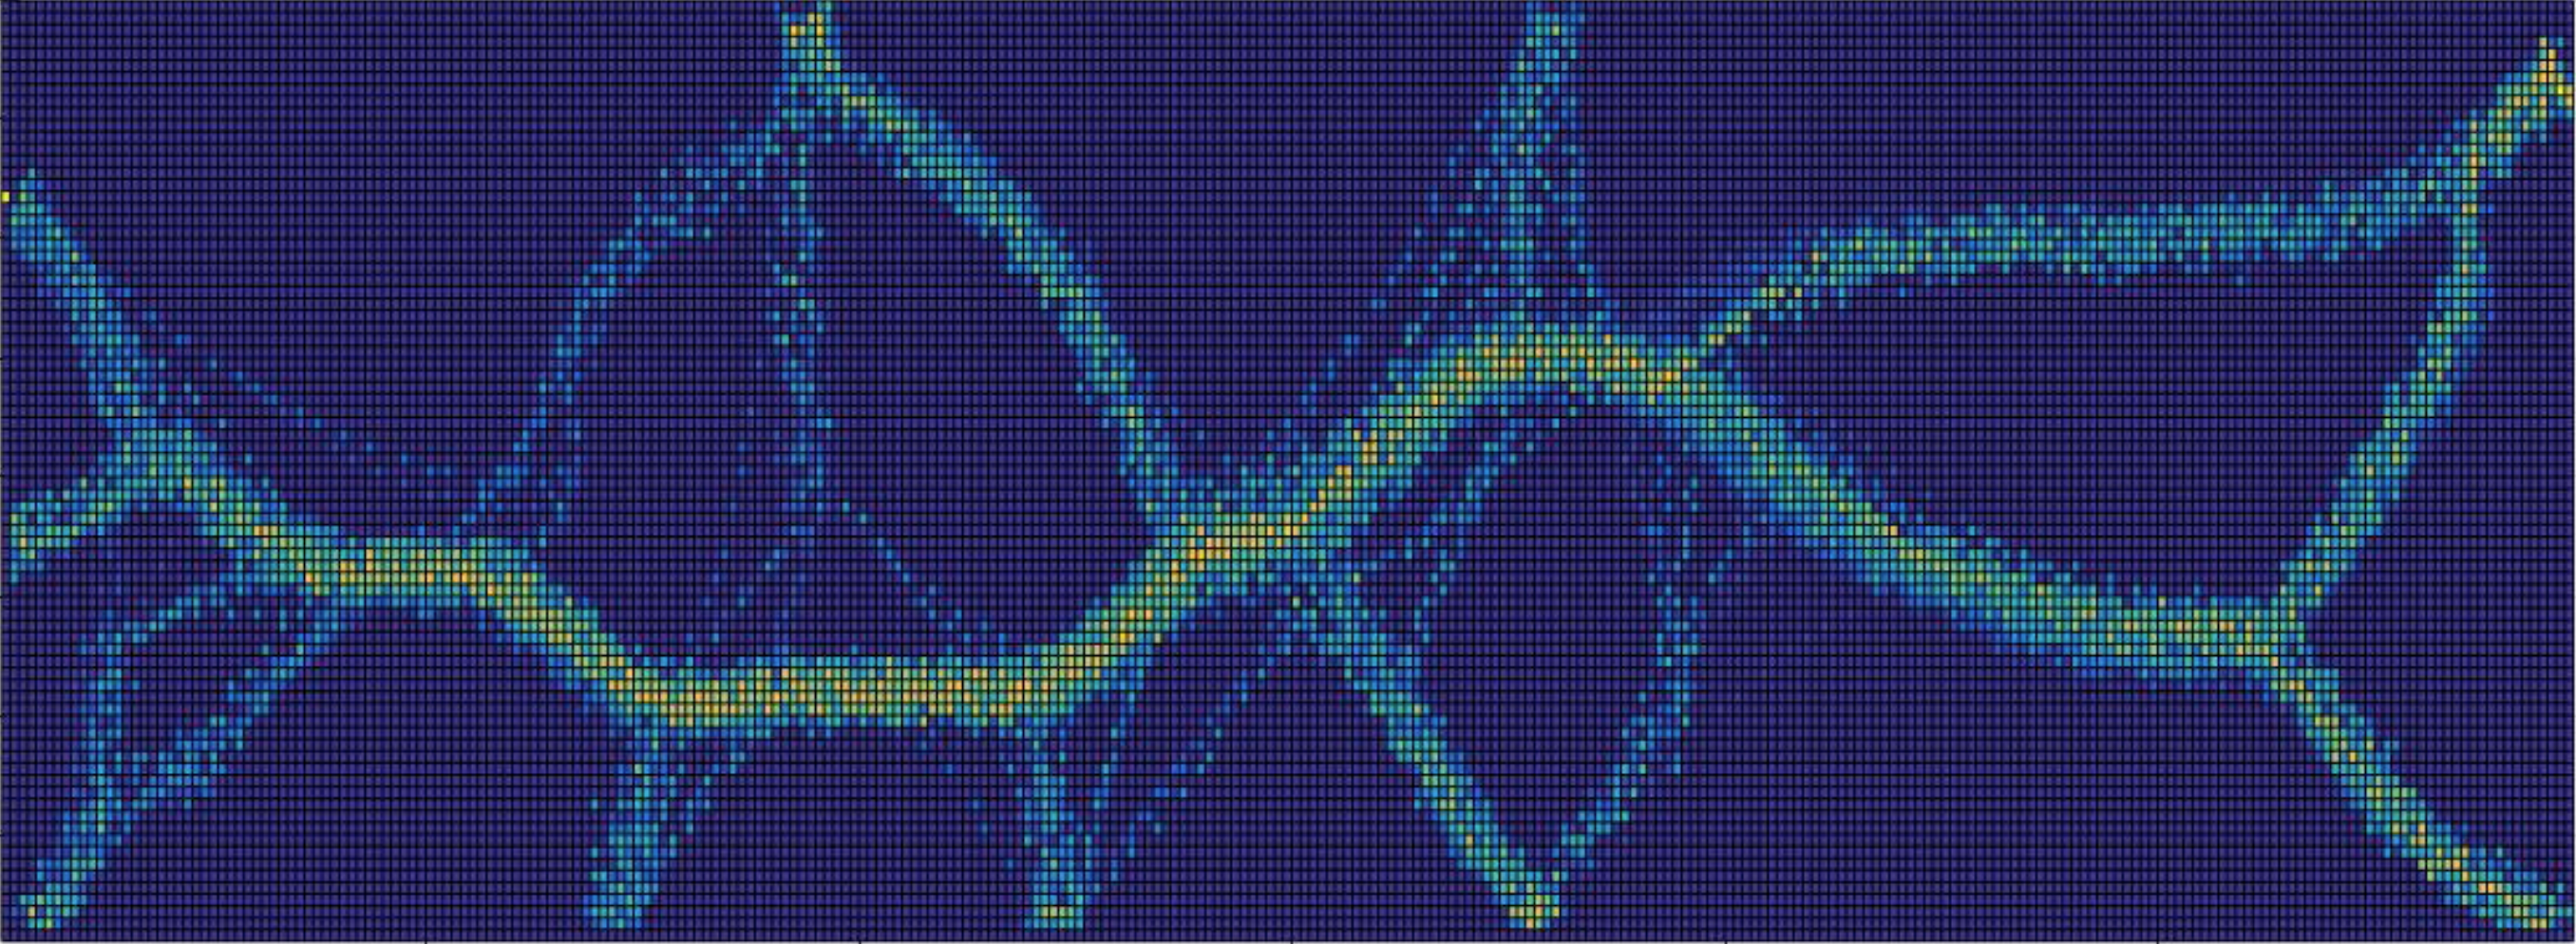
\includegraphics[width=\columnwidth]{jp4.png}
        \caption{Simulation on Joyce Park after 7000 iterations}
        \label{jp4}
\end{figure}

Going to the end, also on the right side the streets changed to one single big street with the links to entrances/exits. The only change till the end is only the "triangle" on the right of the park, that closes to a single crossing. 

\begin{figure}[H]
        \centering
        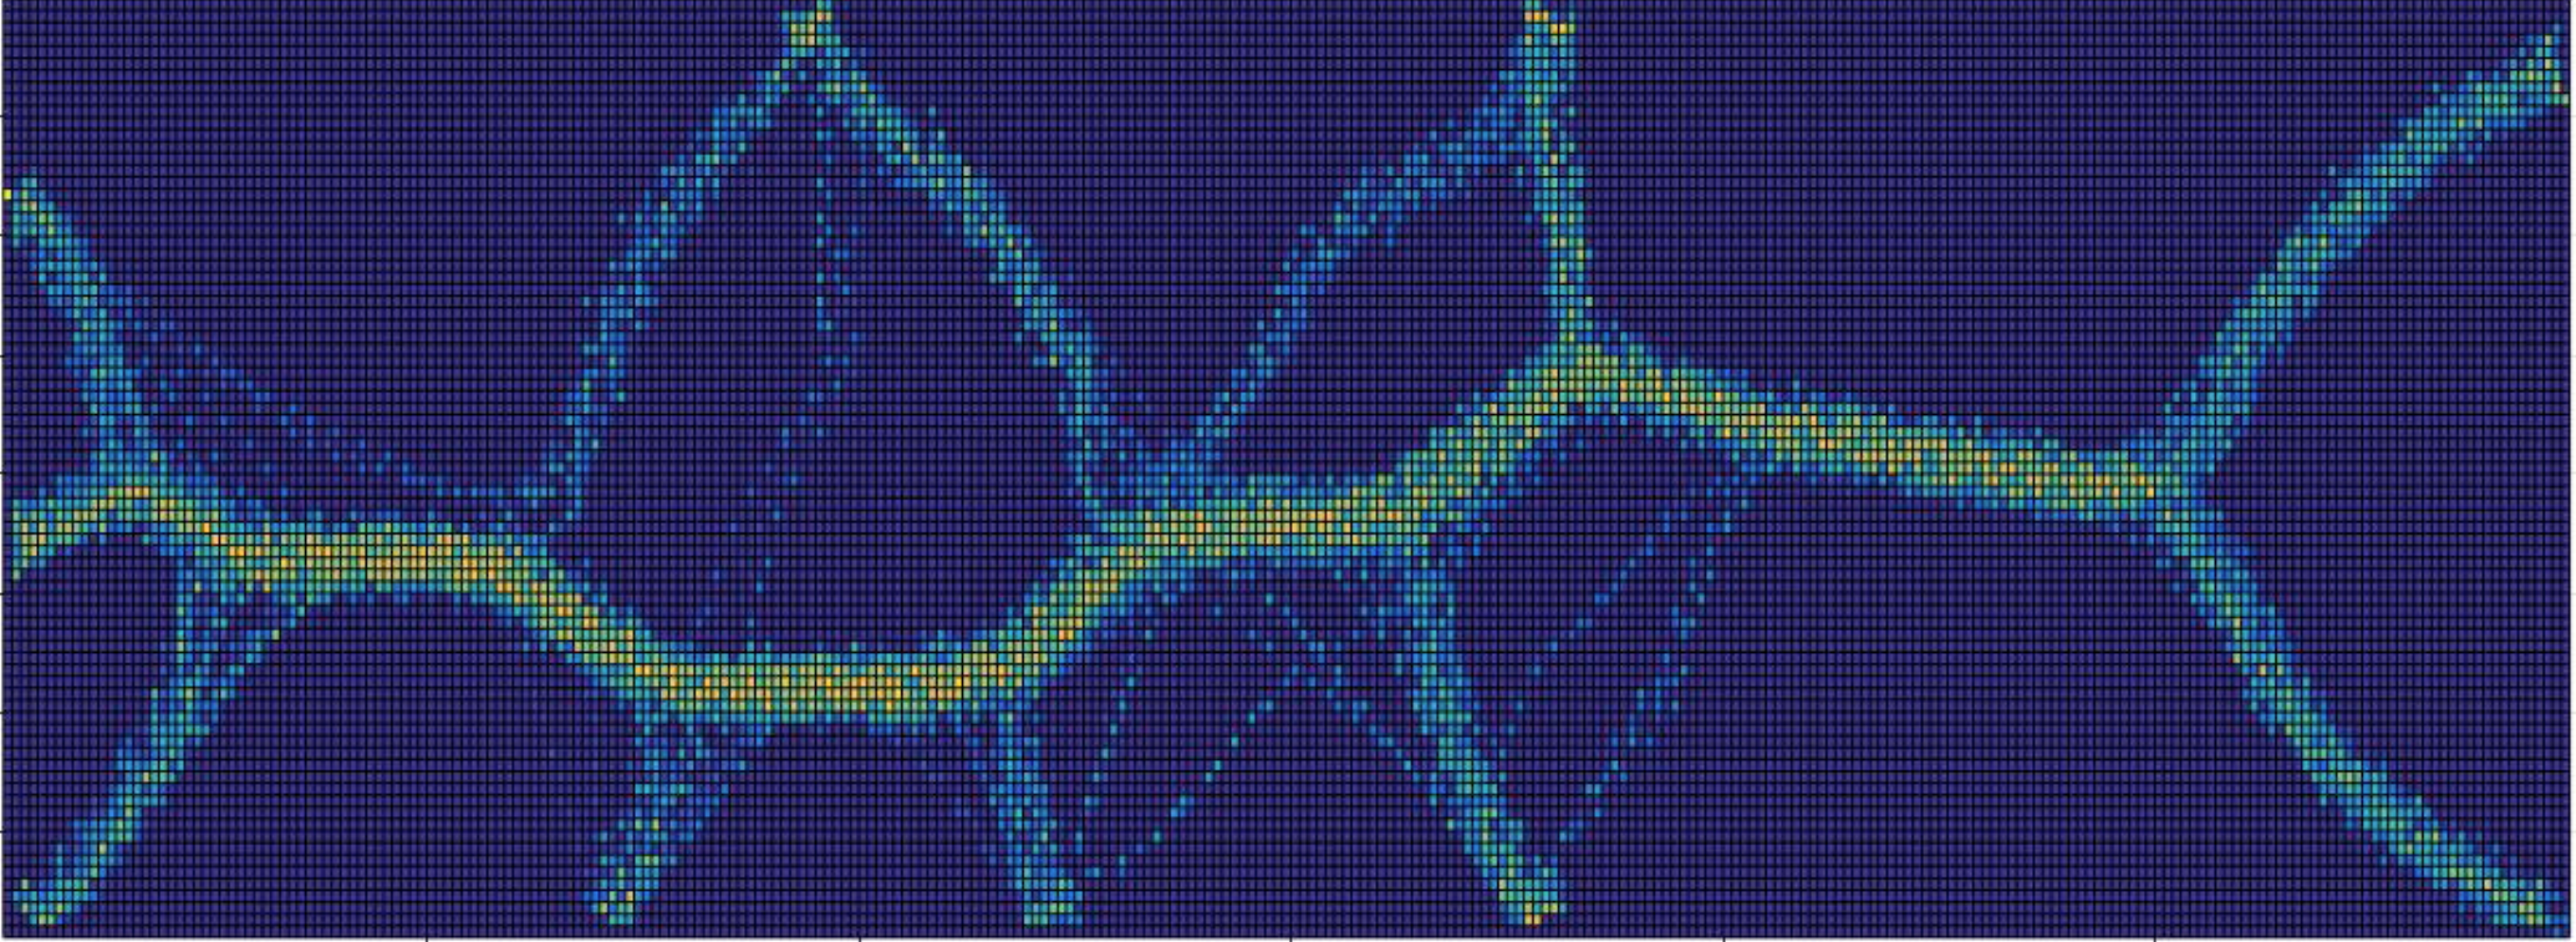
\includegraphics[width=\columnwidth]{jp5.png}
        \caption{Simulation on Joyce Park at the end}
        \label{jp5}
\end{figure}

How we can see in the video at the end the network is stable and there is no modification in the last $2'000$ iterations. However there are still some peoples walking across the park without following the present trails. We think that this behavior is realistic since also in a real park not all peoples follow the trails, but crosses the green areas. 

\newpage

\section{Summary and Outlook}

The work for this project was extremely interesting at the beginning, we had a lot of fun implementing our model and trying to find solutions to the problems. However going to the end, while waiting that the computer performed all the simulations, it became a little bit boring. 
\medskip

During our work, we encountered a lot of difficulties, some of them are listed below:
\begin{itemize}
\item We had some problems implementing the code that compute the potential of the ground. 
\item Solved the first problem our model become very slow, we partially solved it by adding some "if" in order to avoid useless calculus, although it remained slow. The last simulation took almost a week to perform. That was the factor which did not allow us to make another simulation. 
\end{itemize}

\bigskip

The target of an ongoing project could be to make the model more realistic and faster. There are a lot of possibilities to achieve this goal.
Some suggestions:
\begin{itemize}
\item Reanalyze our model of the topology and improve it
\item To take into account that on certain areas of a park can not be walked on
\item Implement also a "social-force" model. It would so be able to simulate also the behavior of peoples in the case that there is a high concentration of pedestrians. 
\end{itemize}

For sure further interesting results could be made by simply changing some parameters and finding data about the percentage of pedestrians entering and going out by the single entrance/exit.




\newpage
\section{References}

\begin{thebibliography}{9}
\bibitem{Modelling Evolution of Human Trail Systems} Modelling Evolution of Human Trail Systems - Dirk Helbing 1997.
\bibitem{book} Camazin 2001 - chapter 13
\end{thebibliography}


\newpage
\appendix
\section{Code}

\subsection{'start.m'}

\begin{lstlisting}

%...................................................
%.................First simulation..................
%...................................................

clear;
clc;
N=1; % Number of simulation

%......... Dimension of matrix

dm = 50; % x dimension
dn = 50; % y dimension

%......... Initial ground condition

G1 = zeros(dm,dn); % Topology

G2 = zeros(dm,dn); % Initial trails
% load ('Trail_1.mat'); % If you want initial presence of trails
% G2=Trail_1;

%.......... Entrance and exits

num_ent=4; % Number of entrance/exits (min N=1 ; max N=4)

% Coordinate have to be between 1 and dm for x, 1 and dn for y

E1v = [1,1]; % Coordinates entrance 1
E2v = [1,49]; % Coordinates entrance 2
E3v = [49,49]; % Coordinates entrance 3
E4v = [49,1]; % Coordinates entrance 4

U1v = [1,1]; % Coordinates exit 1
U2v = [1,49]; % Coordinates exit 2
U3v = [49,49]; % Coordinates exit 3
U4v = [49,1]; % Coordinates exit 4

%.......... Parameters

R = 0.5; % regeneration ratio
I = 30; % Intensity of footprints
v = 3; % Velocity
l=0.8; % Parameter of direction
sigma = 4; % Visibility
iter= 2000; % Number of iteration
dt = 0.1; % Unit of time

%........... Save video and final trails

video_name='Quadrato_1__I30-si4-l0.8-it2000.avi'; % Video name
trail_name='Quadrato_1__I30-si4-l0.8-it2000.mat'; % Name of the final matrix of trails

main % start simulation



%...................................................
%.................Second simulation..................
%...................................................

clear;
clc;
N=2; % Number of simulation

%......... Dimension of matrix

dm = 70; % x dimension
dn = 70; % y dimension

%......... Initial ground condition

G1 = zeros(dm,dn); % Topology

G2 = zeros(dm,dn); % Initial trails
% load ('Trail_1.mat'); % If you want initial presence of trails
% G2=Trail_1;

%.......... Entrance and exits

num_ent=4; % Number of entrance/exits (min N=1 ; max N=4)

% Coordinate have to be between 1 and dm for x, 1 and dn for y

E1v = [35,70]; % Coordinates entrance 1
E2v = [35,1]; % Coordinates entrance 2
E3v = [1,35]; % Coordinates entrance 3
E4v = [70,35]; % Coordinates entrance 4

U1v = [35,70]; % Coordinates exit 1
U2v = [35,1]; % Coordinates exit 2
U3v = [1,35]; % Coordinates exit 3
U4v = [70,35]; % Coordinates exit 4

%.......... Parameters

R = 0.5; % regeneration ratio
I = 10; % Intensity of footprints
v = 3; % Velocity
l=0.8; % Parameter of direction
sigma = 4; % Visibility
iter= 2000; % Number of iteration
dt = 0.1; % Unit of time

%........... Save video and final trails

video_name='Quadrato_2__I10-si4-l0.8-it2000.avi'; % Video name
trail_name='Quadrato_2__I10-si4-l0.8-it2000.mat'; % Name of the final matrix of trails

main % start simulation

%...................................................
%.................Third simulation..................
%...................................................

clear;
clc;
N=3; % Number of simulation

%......... Dimension of matrix

dm = 70; % x dimension
dn = 70; % y dimension

%......... Initial ground condition

G1 = zeros(dm,dn); % Topology

G2 = zeros(dm,dn); % Initial trails
% load ('Trail_1.mat'); % If you want initial presence of trails
% G2=Trail_1;

%.......... Entrance and exits

num_ent=3; % Number of entrance/exits (min N=1 ; max N=4)

% Coordinate have to be between 1 and dm for x, 1 and dn for y

E1v = [2,70]; % Coordinates entrance 1
E2v = [2,1]; % Coordinates entrance 2
E3v = [70,35]; % Coordinates entrance 3
E4v = [90,45]; % Coordinates entrance 4

U1v = [2,70]; % Coordinates exit 1
U2v = [2,1]; % Coordinates exit 2
U3v = [70,35]; % Coordinates exit 3
U4v = [90,45]; % Coordinates exit 4

%.......... Parameters

R = 0.5; % regeneration ratio
I = 30; % Intensity of footprints
v = 3; % Velocity
l=0.8; % Parameter of direction
sigma = 4; % Visibility
iter= 2000; % Number of iteration
dt = 0.1; % Unit of time

%........... Save video and final trails

video_name='Triangolo_1__I10-si4-l0.8-it2000.avi'; % Video name
trail_name='Triangolo_1__I10-si4-l0.8-it2000.mat'; % Name of the final matrix of trails

main % start simulation

%...................................................
%.................Fourth simulation..................
%...................................................

clear;
clc;
N=4; % Number of simulation

%......... Dimension of matrix

dm = 70; % x dimension
dn = 70; % y dimension

%......... Initial ground condition

G1 = zeros(dm,dn); % Topology

G2 = zeros(dm,dn); % Initial trails
% load ('Trail_1.mat'); % If you want initial presence of trails
% G2=Trail_1;

%.......... Entrance and exits

num_ent=2; % Number of entrance/exits (min N=1 ; max N=4)

% Coordinate have to be between 1 and dm for x, 1 and dn for y

E1v = [1,25]; % Coordinates entrance 1
E2v = [1,45]; % Coordinates entrance 2
E3v = [1,45]; % Coordinates entrance 3
E4v = [90,45]; % Coordinates entrance 4

U1v = [90,45]; % Coordinates exit 1
U2v = [90,25]; % Coordinates exit 2
U3v = [1,45]; % Coordinates exit 3
U4v = [90,45]; % Coordinates exit 4

%.......... Parameters

R = 0.5; % regeneration ratio
I = 10; % Intensity of footprints
v = 3; % Velocity
l=0.8; % Parameter of direction
sigma = 4; % Visibility
iter= 2000; % Number of iteration
dt = 0.1; % Unit of time

%........... Save video and final trails

video_name='Parallele_1__I10-si4-l0.8-it2000.avi'; % Video name
trail_name='Parallele_1__I10-si4-l0.8-it2000.mat'; % Name of the final matrix of trails

main % start simulation
\end{lstlisting}

\subsection{'main.m'}

\begin{lstlisting}
G3 = zeros(dm,dn); % presence of peoples
G4 = zeros(dm,dn); % potenzial of ground
G5 = zeros(dm,dn); % slope of ground
M(:,:,1) = G1;
M(:,:,2) = G2;
M(:,:,3) = G3;
M(:,:,4) = G4;
M(:,:,5) = G5;

E = zeros(dm,dn); % entrance
E(E1v(1),E1v(2))=1;
E(E2v(1),E2v(2))=1;
E(E3v(1),E3v(2))=1;
E(E4v(1),E4v(2))=1;

U = zeros(dm,dn); % exits
U(U1v(1),U1v(2))=1;
U(U2v(1),U2v(2))=1;
U(U3v(1),U3v(2))=1;
U(U4v(1),U4v(2))=1;

num_per=0; % Number of peoples

fig = figure('Position',[100 1 1200 900]);

 
vidObj = VideoWriter(video_name);
open(vidObj);

for i=2:iter
    
    change_ground; %modify ground
   
    if(mod(i,4)==2) %insert peoples
        if (num_ent==1)
            insert_person_1_entrance_1_exit;
        end
        if (num_ent==2)
            insert_person_2_entrance_2_exit;
        end
        if (num_ent==3)
            insert_person_3_entrance_3_exit;
        end
        if (num_ent==4)
            insert_person_4_entrance_4_exit;
        end
    end
    
    direction_pend; % calculate best direction
    move_person; % moves peoples
    
    hold off;
    surf(M(:,:,2))
    view(2)
    currFrame = getframe;   % Write each frame to the file.
    writeVideo(vidObj,currFrame);
    [N,i]
end

close(vidObj); % Close the file.
close all
PR1 = M(:,:,2);
save (trail_name,'PR1'); 
\end{lstlisting}

\subsection{'change\_ground.m'}

\begin{lstlisting}
for j=1:dm
    for k=1:dn
        if(M(j,k,3) == 1) % if there is a person
            dG = -R*M(j,k,2)*dt + I*(1 - M(j,k,2))*dt;
            M(j,k,2) = M(j,k,2) + dt*dG;
        else
            dG = -R*M(j,k,2)*dt;
            M(j,k,2) = M(j,k,2) + dt*dG;
        end
    end
end
\end{lstlisting}

\subsection{'insert\_person\_1\_entrance\_1\_exit.m'}

\begin{lstlisting}
num_per= num_per +1;

M(E1v(1),E1v(2),3)=1;
P(num_per,:)=[E1v(1),E1v(2),U1v(1),U1v(2),0];
\end{lstlisting}

\subsection {'insert\_person\_2\_entrance\_2\_exit.m'}

\begin{lstlisting}
h = rand;
o = rand;
num_per= num_per +1;

if (h<=0.5) %Entrance 1
    M(E1v(1),E1v(2),3)=1;
    P(num_per,:)=[E1v(1),E1v(2),U2v(1),U2v(2),0]; %Exit 2
end

if (h>0.5) %Entrance 2
    M(E2v(1),E2v(2),3)=1;
    P(num_per,:)=[E2v(1),E2v(2),U1v(1),U1v(2),0]; %Exit 1
end
\end{lstlisting}

\subsection {'insert\_person\_3\_entrance\_3\_exit.m'}

\begin{lstlisting}
h = rand;
o = rand;
num_per= num_per +1;

if (h<=0.33) %Entrance 1
    M(E1v(1),E1v(2),3)=1;
    if (o<=0.5) %Exit 2
        P(num_per,:)=[E1v(1),E1v(2),U2v(1),U2v(2),0];
    end
    if (o>0.5) %Exit 3
        P(num_per,:)=[E1v(1),E1v(2),U3v(1),U3v(2),0];
    end
end

if (h>0.33 && h<=0.66) %Entrance 2
    M(E2v(1),E2v(2),3)=1;
    if (o<0.5) %Exit 1
        P(num_per,:)=[E2v(1),E2v(2),U1v(1),U1v(2),0];
    end
    if (o>=0.5) %Exit 3
        P(num_per,:)=[E2v(1),E2v(2),U3v(1),U3v(2),0];
    end
end

if (h>0.66) %Entrance 3
    M(E3v(1),E3v(2),3)=1;
    if (o<=0.5) %Exit 1
        P(num_per,:)=[E3v(1),E3v(2),U1v(1),U1v(2),0];
    end
    if (o>0.5) %Exit 2
        P(num_per,:)=[E3v(1),E3v(2),U2v(1),U2v(2),0];
    end
end
\end{lstlisting}

\subsection {'insert\_person\_4\_entrance\_4\_exit.m'}

\begin{lstlisting}
h = rand;
o = rand;
num_per= num_per +1;

if (h<=0.25) %Entrance 1
    M(E1v(1),E1v(2),3)=1;
    if (o<=0.33) %Exit 2
        P(num_per,:)=[E1v(1),E1v(2),U2v(1),U2v(2),0];
    end
    if (o>0.33 && o<=0.66) %Exit 3
        P(num_per,:)=[E1v(1),E1v(2),U3v(1),U3v(2),0];
    end
    if (o>0.66) %Exit 4
        P(num_per,:)=[E1v(1),E1v(2),U4v(1),U4v(2),0];
    end
end


if (h>0.25 && h<=0.5) %Entrance 2
    M(E2v(1),E2v(2),3)=1;
    if (o<=0.33) %Exit 1
        P(num_per,:)=[E2v(1),E2v(2),U1v(1),U1v(2),0];
    end
    if (o>0.33 && o<=0.66) %Exit 3
        P(num_per,:)=[E2v(1),E2v(2),U3v(1),U3v(2),0];
    end
    if (o>0.66) %Exit 4
        P(num_per,:)=[E2v(1),E2v(2),U4v(1),U4v(2),0];
    end
end

if (h>0.5 && h<=0.75) %Entrance 3
    M(E3v(1),E3v(2),3)=1;
    if (o<=0.33) %Exit 1
        P(num_per,:)=[E3v(1),E3v(2),U1v(1),U1v(2),0];
    end
    if (o>0.33 && o<=0.66) %Exit 2
        P(num_per,:)=[E3v(1),E3v(2),U2v(1),U2v(2),0];
    end
    if (o>0.66) %Exit 4
        P(num_per,:)=[E3v(1),E3v(2),U4v(1),U4v(2),0];
    end
end

if (h>0.75) %Entrance 4
    M(E4v(1),E4v(2),3)=1;
    if (o<=0.33) %Exit 1
        P(num_per,:)=[E4v(1),E4v(2),U1v(1),U1v(2),0];
    end
    if (o>0.33 && o<=0.66) %Exit 2
        P(num_per,:)=[E4v(1),E4v(2),U2v(1),U2v(2),0];
    end
    if (o>0.66) %Exit 3
        P(num_per,:)=[E4v(1),E4v(2),U3v(1),U3v(2),0];
    end
end

\end{lstlisting}

\subsection {'move\_person.m'}

\begin{lstlisting}
for n=1:num_per
     if(P(n,5)==0)
        vrand = (rand + 0.5)*v;
        sx = round(ealfa(n,1)*vrand);
        sy = round(ealfa(n,2)*vrand);
        M(P(n,1),P(n,2),3) = 0;
        if ((P(n,1) + sx)>= dm || (P(n,2) + sy)>= dn || (P(n,1) + sx)<= 1  || (P(n,2) + sy)<=1)
             M(P(n,1),P(n,2),3) = 0;
             clearvars P(n);
             P(n,5)=1;
        else
             P(n,1) = P(n,1) + sx;
             P(n,2) = P(n,2) + sy;
        end

        M((P(n,1)),(P(n,2)),3) = 1;
     else
         M(P(n,1),P(n,2),3) = 0;
     end
end
\end{lstlisting}

\subsection{'direction\_pend.m'}

\begin{lstlisting}

for aa=1 : dm   % for that goes trough the matrix
    for bb=1:dn
        pottot=0; %sum of all potential with respect to point [aa bb]
        for q=1:dm
            for w=1:dn
                if (M(q,w,2)~=0)
                    pot = M(q,w,2)*exp(-((aa-q)^2 + (bb-w)^2)^(1/2)/sigma);%potential of the ground in [q w] respect to [aa bb]
                    pottot=pottot+ pot; %sum of all potentials
                end
            end
        end
        pottot = pottot/(dm*dn); %avarage
        M(aa,bb,4)=pottot; %putting the potential in the matrix crated for it  
    end
end

for n=1:num_per  % for all peoples
    if (P(n,5)==0)  % peoples that are not "cancelled"
        
        pot_per = M(:,:,4);
        
        for q=1:dm
            for w=1:dn
                dist = ((P(n,1)-q)^2 + (P(n,2)-w)^2)^(1/2); %distance
                if (dist ~=0)
                    pend = (1000*M(q,w,1) - M(P(n,1),P(n,2),1))/dist; %slope
                    if (pend < 0)
                        pot_per(q,w) = M(q,w,4) - exp(1/pend);
                    elseif (pend > 0)
                        pot_per(q,w) = M(q,w,4) - exp(-1/pend);
                    else
                        pot_per(q,w) = M(q,w,4);
                    end
                else
                    pot_per(q,w) = M(q,w,4);
                end
            end
        end
        
        [fy,fx]=gradient(pot_per(:,:));  % gradient of the potential matrix
        
        gradnorm = ((fx(P(n,1),P(n,2)))^2 + (fy(P(n,1),P(n,2)))^2)^(1/2);
        
        distmeta=((P(n,3) - P(n,1))^2 + (P(n,4) - P(n,2))^2)^(1/2); %distance from target
        
        if (distmeta >=1)
            
            if (gradnorm ~= 0)
                ex = (P(n,3) - P(n,1))/distmeta + fx(P(n,1),P(n,2))*l/gradnorm;
                ey = (P(n,4) - P(n,2))/distmeta + fy(P(n,1),P(n,2))*l/gradnorm;
            else
                ex = (P(n,3) - P(n,1))/distmeta;
                ey = (P(n,4) - P(n,2))/distmeta;
            end
            norm = (ex^2 + ey^2)^(1/2);
        else
            M(P(n,1),P(n,2),3) = 0;
            clearvars P(n);
            P(n,5)=1;
        end     
        ealfa(n,:) = [ex/norm,ey/norm]; % direction vector     
    end
end
\end{lstlisting}


\end{document}  



 
